% !TeX root = ../my-thesis.tex
\chapter{Grundlagen}

\section{Datenschutzkriterien}
\subsection{IT-Grundschutz}
Der IT-Grundschutz definiert den Schutzbedarf eines bestimmten Assets je nachdem welches Risiko bei Verletzung der Grundwerte Vertraulichkeit, Integrität und Verfügbarkeit entstehen [10]. Allgemein existieren folgende Schutzbedarfskategorien:
\begin{itemize} 
\item \textbf{normal} (Schadenauswirkungen begrenzt bis überschaubar)
\item \textbf{hoch} (Schadenauswirkungen könnten hoch bzw. beträchtlich sein)
\item \textbf{sehr hoch} (Schadensauswirkungen können ein existenziell bedrohliches Ausmaß annehmen
\end{itemize}
Bei dem Authentifikationsprototypen wird die Schadensauswirkung für alle nicht personenbezogenen Daten wohl im Bereich normal liegen, da schon im Aufbau darauf geachtet wird, dass nur so viele Daten vom User verwendet werden, wie zwingend notwendig. (Nach dem Need-To-Know Prinzip) Sollte die Webseite oder Teile der Webseite publiziert bzw. im Business - Umfeld genutzt werden, muss eine Neubewertung der Daten nach Vertraulichkeit, Integrität und Verfügbarkeit stattfinden. Vor allem muss darauf geachtet sein, dass Daten über Fingerabdrücke verschlüsselt und Passwörter im gehashten Zustand in Datenbanken persistiert werden. Bei Kompromittierung des Hauptrechners, welches die größte Bedrohung in diesem Szenario darstellen würde, droht ein Data Breach mit dem Angreifer diese Daten weiterverwenden können. Durch Verschlüsselungen durch Schlüssel, die nicht auf dem Hauptsystem (oben u.a als Hauptrechner benannt) liegen. Gleichzeitig sollten die genutzten Verfahren insgesamt mathematisch sicher sein, auf veraltete Verschlüsselungsverfahren ist zu verzichten. Dies gillt auch für Hashes wie MD5, die mittlerweile relativ akkurat durch sehr große vorgerechnete Tabellen erraten werden können. \newpage

Im Falle einer Kompromittierung besäße der Schutzbedarf der Daten innerhalb der Datenbank, welche nicht gehasht oder anderweitig verschlüsselt sind, die Kategorie 'sehr hoch'. Eine Kompromittierung kann für das Unternehmen einen Imageschaden sowie weitreichende juristische Klagen zur Folge haben. Damit sind bereits 2 der 7 aufgeführten Schadensszenarien durch den \ac{bsi} beschrieben. Je nach dem wie kompliziert die Ursprungsdaten sind und welcher Hashingalgorithmus in Kombination mit Salt und Pepper genutzt wurde, können vorallem Nutzerpassphrasen an die Öffentlichkeit gelangen und Angreifer können die Passwörter für andere Dienste nutzen. Die Wahrscheinlichkeit für diesen Schaden ist noch vergleichbar niedrig, weshalb die Schadensauswirkung hoch statt sehr hoch ist. \\ \\
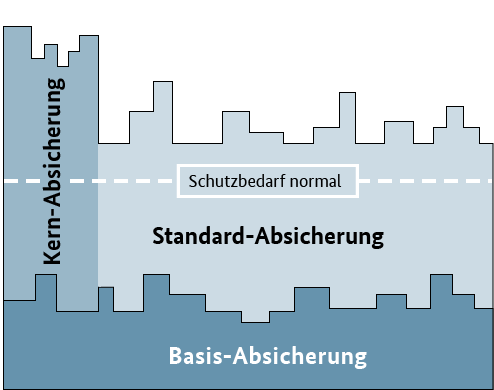
\includegraphics[width=15cm]{Abb_2_09_Varianten.png} \\
\\
Der IT-Grundschutz definiert drei Arten der Absicherung. Die Basis-Absicherung ist relevant für Institutionen die einen Einstieg in den IT-Grundschutz suchen und relativ schnell alle relevanten Geschäftspozesse mit einfach umzusetzenden Basismaßnahmen sichern wollen. Die Kern-Absicherung konzentriert sich auf besonders wichtige Geschäftsprozesse und vertieft sich in die Sicherung dieser. Von einer Standard-Absicherung spricht man, wenn alle empfohlenen IT-Grundschutz-Vorgehensweisen durchgeführt werden. Sie beschreibt den allumfassenden Schutz der Prozesse und Bereiche der Institution, wie das Schaubild vom BSI verdeutlicht. [9] Bei dem Prototyp wird eine Basis-Absicherung nach BSI durchgeführt und darauf geachtet alle Datenschutzkriterien zu erfüllen. Dabei wird vor allem die Checkliste des IT-Grundschutzes zu Webservern und Webanwendungen betrachtet. Kriterien die nicht erfüllt werden konnten oder wurden, werden dokumentiert und im Fazit erläutert. Die Wahl der Basis-Absicherung begründet sich damit, das lokale Testdaten im Prototyp verarbeitet werden, für die kein bis nur ein sehr geringer Schutzbedarf besteht. Eine Kern-Absicherung käme nur in Frage, falls ein ganz bestimmter Prozess oder Asset des Prototyps geschützt werden müsste wie zum Beispiel der Zugriff auf die Datenbank durch den Prototypen, welche nicht der Fall ist. Insgesamt ist dieser Teil der Abschlussarbeit auch als Einstieg in den IT-Grundschutz zu verstehen, welcher laut BSI selbst die Basis-Absicherung als Empfehlung und zur Folge meiner Entscheidung hat und sich am Besten für vorhandene Zwecke eignet.

\subsection{ISO 27001}
Zunächst einmal muss unterschieden werden zwischen dem Standard ISO 27001 und der Zertifizierung von ISO 27001 auf Basis des IT - Grundschutzes. Im Grundansatz sind diese beiden Ansätze soweit kompatibel, da sie beide ein \ac{isms} beschreiben, um Risiken in der Informationssicherheit zu dezimieren (oder im besten Fall zu eliminieren). Im Buch 'Das ISMS nach 27001' beschreiben die Autoren Heinrich Kersten, Jürgen Reuter und Klaus-Werner Schröder das ISMS als ``ein spezialisiertes System, in dessen Fokus die Wahrung der Informationssicherheit steht'' [11]. \\\\
Beide Standards beschreiben eine Kontinuität in der regelmäßigen Überprüfung und Neubewertung der Risiken für die Institution. Ein wesentlicher Unterschied zwischen ihnen liegt in der Risikoanalyse. Während beim BSI-Grundschutz eine Risikoanalyse nur in besonderen Fällen erforderlich ist, ist sie beim Standard ISO 27001 ein fester Bestandteil, an das keine Bedingungen geknüpft sind. Wobei streng genommen häufig der eigentliche Schriftzug zur Risikoanalyse in der Norm ISO 27005 steht und darauf häufig verwiesen wird. Gleichzeitig sei laut Dr. Markus a Campo der Standard ISO 27001 mehr an dem Management der Informationssicherheit interessiert, wogegen der BSI-Grundschutz sich auf die detaillierte Vorgehensweise zur Minimierung von Risiken stütze. Unabhängig vom gewählten Standard sei es außerdem sinnvoll, die eigene Sicherheit in regelmäßigen Abständen zu überprüfen.
Laut dem \ac{bsi} ist die ISO 27001 Zertifizierung auf Basis des IT-Grundschutzes für sowohl Standard als auch die Kern-Absicherung möglich. [8] \\\\

\section{Authentifizierungsmethoden}
\subsection{Username \& Passwort}
Trotz der bereits erwähnten Unsicherheiten und Probleme des beliebten Schlüssels aus der Kategorie Wissen, dem Passwort, ist das Passwort laut eines Artikels von Thomas Maus 2008 ``nicht aus unserer Arbeitswelt [...] wegzudenken'' [12] Der Artikel spricht bereits 2008 über alternative Authentifikationsmethoden wie der Einmalkennwörter und Weiterem. Dies ist nur ein weiterer Beweis dafür, dass schon vor mehr als 10 Jahren die Passwortproblematik erkannt wurde. In dem Artikel geht Herr Maus der Hypothese nach, ob nun Passwörter wirklich per sé unsicherer sind als die Authentifikationsmethoden der beiden anderen Kategorien Besitz und biologische Merkmale. So sei das Kernproblem des Passwortes, dass das Passwort direkt nach der Eingabe ein geteiltes Geheimnis ist, da alle beteiligten Systeme es nun mitschneiden konnten und nun automatisch Geheimnisträger sind. Das Passwort bietet sehr viele Angriffsvektoren, so ``Shoulder Sourfing, Phishing, Social-Engineering, Man-in-the-Middle Angriffe, schlechte Passwort Qualitäten, das Teilen des Passwortes mit Familie und Freunden'' [12] und vielem mehr. \\
Bei dem Prototyp wird der Ist-Zustand einer Username und Passwort - Authentifikation demonstriert, wie man sie heutzutage auf höchstwahrscheinlich jedem Webdienst in der Form als ersten schwachen Faktor vorfinden wird. Während man über alle Schwächen des Passwortes spricht, muss man dennoch anerkennen, dass das Passwort eine gewisse Flexibilität bietet. Es genügt das Wissen über eine bestimmte Zeichenfolge um sich zu authentifizieren, dieses Wissen muss nicht zwangsmäßig auf ein Blatt geschrieben oder in einem Passwort-Manager beherrbergt werden. Das beste Passwort ist jenes, welches nur in dem Gehirn des Nutzers persistiert ist und mit niemandem geteilt wird. Anders als bei neueren Verfahren, die als sicherer gelten, benötigt es keine Smart-Card, USB-Sticks oder anderweitige technische Hilfsmittel um sich zu authentifizieren.

\subsection{Einmalkennwörter}
Ein Kennwort ist eine "eine Zeichenfolge, die zur Authentifizierung verwendet wird. Damit soll die Identität einer Person [...] auf eine Ressource nachgewiesen werden." \cite{A4}. Ein Einmalkennwort im Vergleich ist ein Kennwort, das nur ein einziges Mal für eine Authentifizierung genutzt werden kann. Man unterscheidet drei Arten von \ac{otp}'s.

\subsubsection{Timerbasiert}
 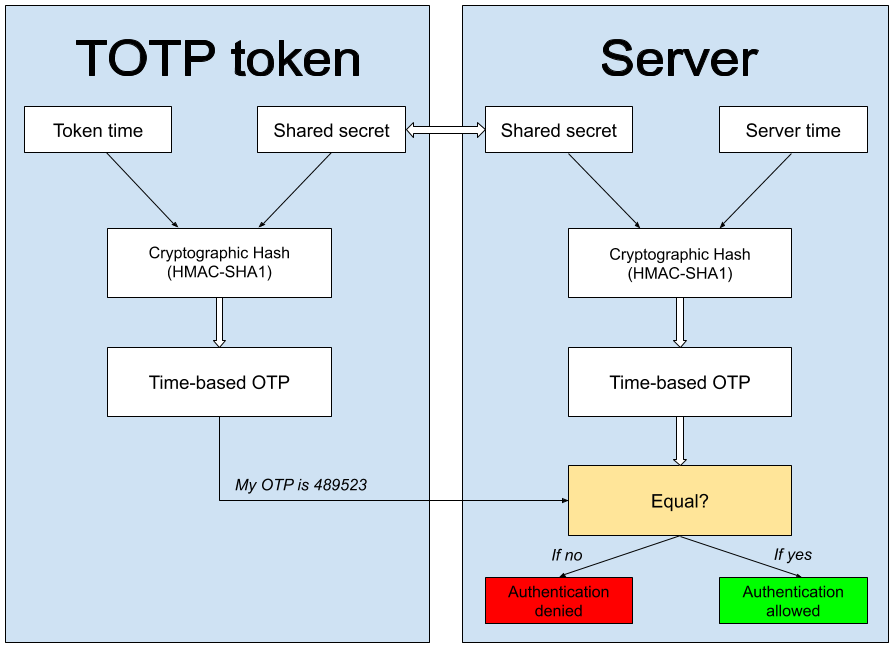
\includegraphics[width=15cm]{TOTP-algorithm-explained.png} \\\\
 Bei der timerbasierten (\ac{totp}) Methode wird die aktuelle Systemzeit (Token time) mit dem zu verschlüsselnden Text (Shared secret) anhand eines kryptografischen Verfahrens verschlüsselt. Es entsteht ein kryptografischer Hashwert (Cryptographic Hash), welcher meist den HMAC-SHA1 Hashingalgorithmus verwendet. Dieses Verfahren findet gleichermaßen auf dem Server statt. Der einzige Unterschied zum Server besteht darin, dass die Systemzeit des Servers genutzt wird. Findet innerhalb der festgelegten Zeit (ein Token entfällt laut RFC6238 standartmäßig nach 30 Sekunden, diese Zeit ist modifizierbar) eine erfolgreiche Authentifikation statt, wird der Zugang gewährt. [13]
 
 Laut Margaret Rouse biete das TOTP Verfahren zusätzliche Sicherheit für den Nutzer, da selbst bei Erhalt des Passwortes das TOTP nicht in die Hände des Angreifers gelangt und nach einer gewissen Toleranzzeit verfällt. (\cite{A5} Eine Beispielapplikation für die Nutzung eines TOTP - Ansatzes für zusätzliche Sicherheit ist der "Google Authenticator", welches in jedem gängigen App Store zu finden ist.

\subsubsection{Ereignisbasiert}
Ereignisbasierte OTPs besitzen einen Ereigniszähler, der bei jeder versuchten Authenzifizierung einen Zähler auf Server und Clientseite synchronisiert inkrementiert. Sollte der Zähler asychnron werden bzw. der Server einen anderen Wert gespeichert haben als der Client bei der nächsten Authentifizierung sendet, wird der Authentifizierungsvorgang abgebrochen. Man findet diese Funktionalität wortwörtlich beschrieben in Googles Time and event based one time password" - Patent \cite{A6} in folgendem Wortlaut "[...] the characteristics of an event can be the value of a counter that is incremented each time the user pushes a button on the token" \cite{A6}. Für diesen Prozess wird der HOTP Algorithmus genutzt, der im RFC4226 näher beschrieben ist. Diese Art der Authentifizierung kann zum Beispiel für die E-Mail Verifikation und damit die Identifikation (wie zuvor erläutert) genutzt werden.
	
\subsubsection{Challenge-response}
Challenge-response basierte OTP Verfahren bedienen sich an komplizierten mathematischen Verfahren. Das heißt, es erfolgt ein ACK (Acknowledge bzw. Initialanstoß zur Authentifizierung). Der Client, berechnet die Response mithilfe der mathematischen Formel und sendet das Ergebnis an den Server. Sollte es einen Match geben, erhält der Client eine Response vom Server, der seine Echtheit bestätigt. Synchronisationsprobleme kann es bei diesem Verfahren entgegen der ereignis oder timerbasierten OTP-Verfahren nicht geben, da die Berechnung dieses 'Schlüssels' vollkommen auf der Clientseite funktioniert. Der Server überprüft diese Rechnung nur mit seinem eigenen Wert, stellt aber keine weiteren Rechnungen oder Umformungen mit diesem Wert an. Der Hauptvorteil dieses Verfahrens ist, dass unabhängig von der Zeit und einem speziellen Ereignis eine Anfrage gestellt werden kann. Der Server kann also seine 'Challenge' abschicken und muss keine 'Response' innerhalb einer festgegebenen Zeit erhalten, um authentifizieren zu können. Dieses Verfahren gilt als besonders sicher, da es auf Serverseite keinen Algorithmus gibt, der sich vorausberechnen lässt.

\subsection{Authentifizierung über Schlüssel}
\subsection{Biometrisierte Authentifizerung}
